\chapter{Recycling High Density Polyethylene for 3D Printing}
\label{Appendix:hdpe}

As the project was nearing the production phase, the Sustainability team proposed a collaboration 
to enhance environmental responsibility. Their suggestion was to explore the feasibility of 3D 
printing the device's enclosure using \textit{High Density Polyethylene} (HDPE), sourced from the 
recycling of chemical containers used by the company for cleaning purposes.

In parallel, they established contact with the ``Centro de Innovación en Economía Circular'' 
(CIEC), a facility owned by the Community of Madrid, dedicated to promoting circular economy 
practices. The CIEC is equipped with a fabrication laboratory (\textit{fablab}) that houses the 
necessary tools for recycling HDPE and converting it into 3D-printable filament.

With the support of the CIEC, the team gained access to the essential equipment for this project. 
The CIEC staff were extremely supportive, providing the machinery and guidance needed on-site, 
free of charge.

This appendix outlines the process of transforming plastic containers into 3D-printable filament. 
The following steps provide a summary of this process, which will be elaborated upon in subsequent 
sections:

\begin{itemize}
    \item \textbf{Initial Preparation}: The first step involves cutting the HDPE containers into 
    smaller pieces that can be fed into a plastic shredder.
    \item \textbf{Shredding}: These pieces are then shredded into fragments smaller than pea-sized 
    particles, with additional post-processing as necessary.
    \item \textbf{Filament Production}: The shredded plastic is fed into a filament-making 
    machine, which is configured to produce the final 3D-printable filament.
\end{itemize}

By repurposing recycled HDPE, this initiative not only supports the project's sustainability goals 
but also demonstrates a practical application of circular economy principles in modern 
manufacturing.

\section{Initial Preparation}

The initial preparation process, although the least time-consuming step in recycling HDPE, is 
crucial to ensure the quality of the final product. Without proper care, the filament produced can 
be contaminated to the point of being unusable.

First, it is essential to ensure that the chemicals previously stored in the containers are 
non-toxic. The team did not have the facilities to properly clean and neutralize hazardous 
chemicals, so containers that held dangerous substances were not used.

Additionally, many containers had visibly dirty sections. Including these contaminated parts in 
the recycling process was found to significantly increase impurities in the final filament. These 
impurities can compromise the print quality and mechanical properties, rendering the filament 
unsuitable for use.

Therefore, meticulous inspection and cleaning of the containers are necessary. All parts that 
cannot be thoroughly cleaned or show signs of significant contamination should be discarded. 
Although this might seem wasteful, ensuring the purity of the HDPE is critical for producing 
high-quality 3D printing filament. Ensuring that only clean, non-toxic containers are used is a 
key step in achieving a successful recycling process.

\section{Shredding and Post-Processing}

Shredding the plastic is straightforward with the \textit{GP20 Plastic Shredder}\footnote{GP20 
Plastic Shredder: \url{https://www.3devo.com/gp20-plastic-shredder}} by \textit{3devo}. However, 
due to HDPE's elastic nature and resistance to breaking apart, the shredder occasionally needed to 
reverse its blades to effectively cut through the material. This happens automatically nonetheless.

Regarding post-processing, most filaments require drying after shredding but before filamenting. 
This is because moisture in the plastic can lead to steam vapor during extrusion, which deforms 
the plastic and ruins the filament roll. Despite this, multiple attempts to remove water from the 
HDPE plastic using 3devo's AIRID dryer\footnote{AIRID dryer: \url{https://www.3devo.com/dryer}} 
yielded negligible results. The weight difference of a 500g bag of shredded filament after drying 
was only 0.5g, resulting in 499.5g, which could be attributed to residual plastic left in the 
dryer and falls within the margin of error.

Given this experimentation, it was concluded that drying the shredded plastic was unnecessary for 
this process. In Figure \ref{fig:shredded_filament}, the final result of the shredding process can 
be seen, and in Figure \ref{fig:shredder_dryer} both machines can be seen.

\begin{figure}[h]
	\centering
	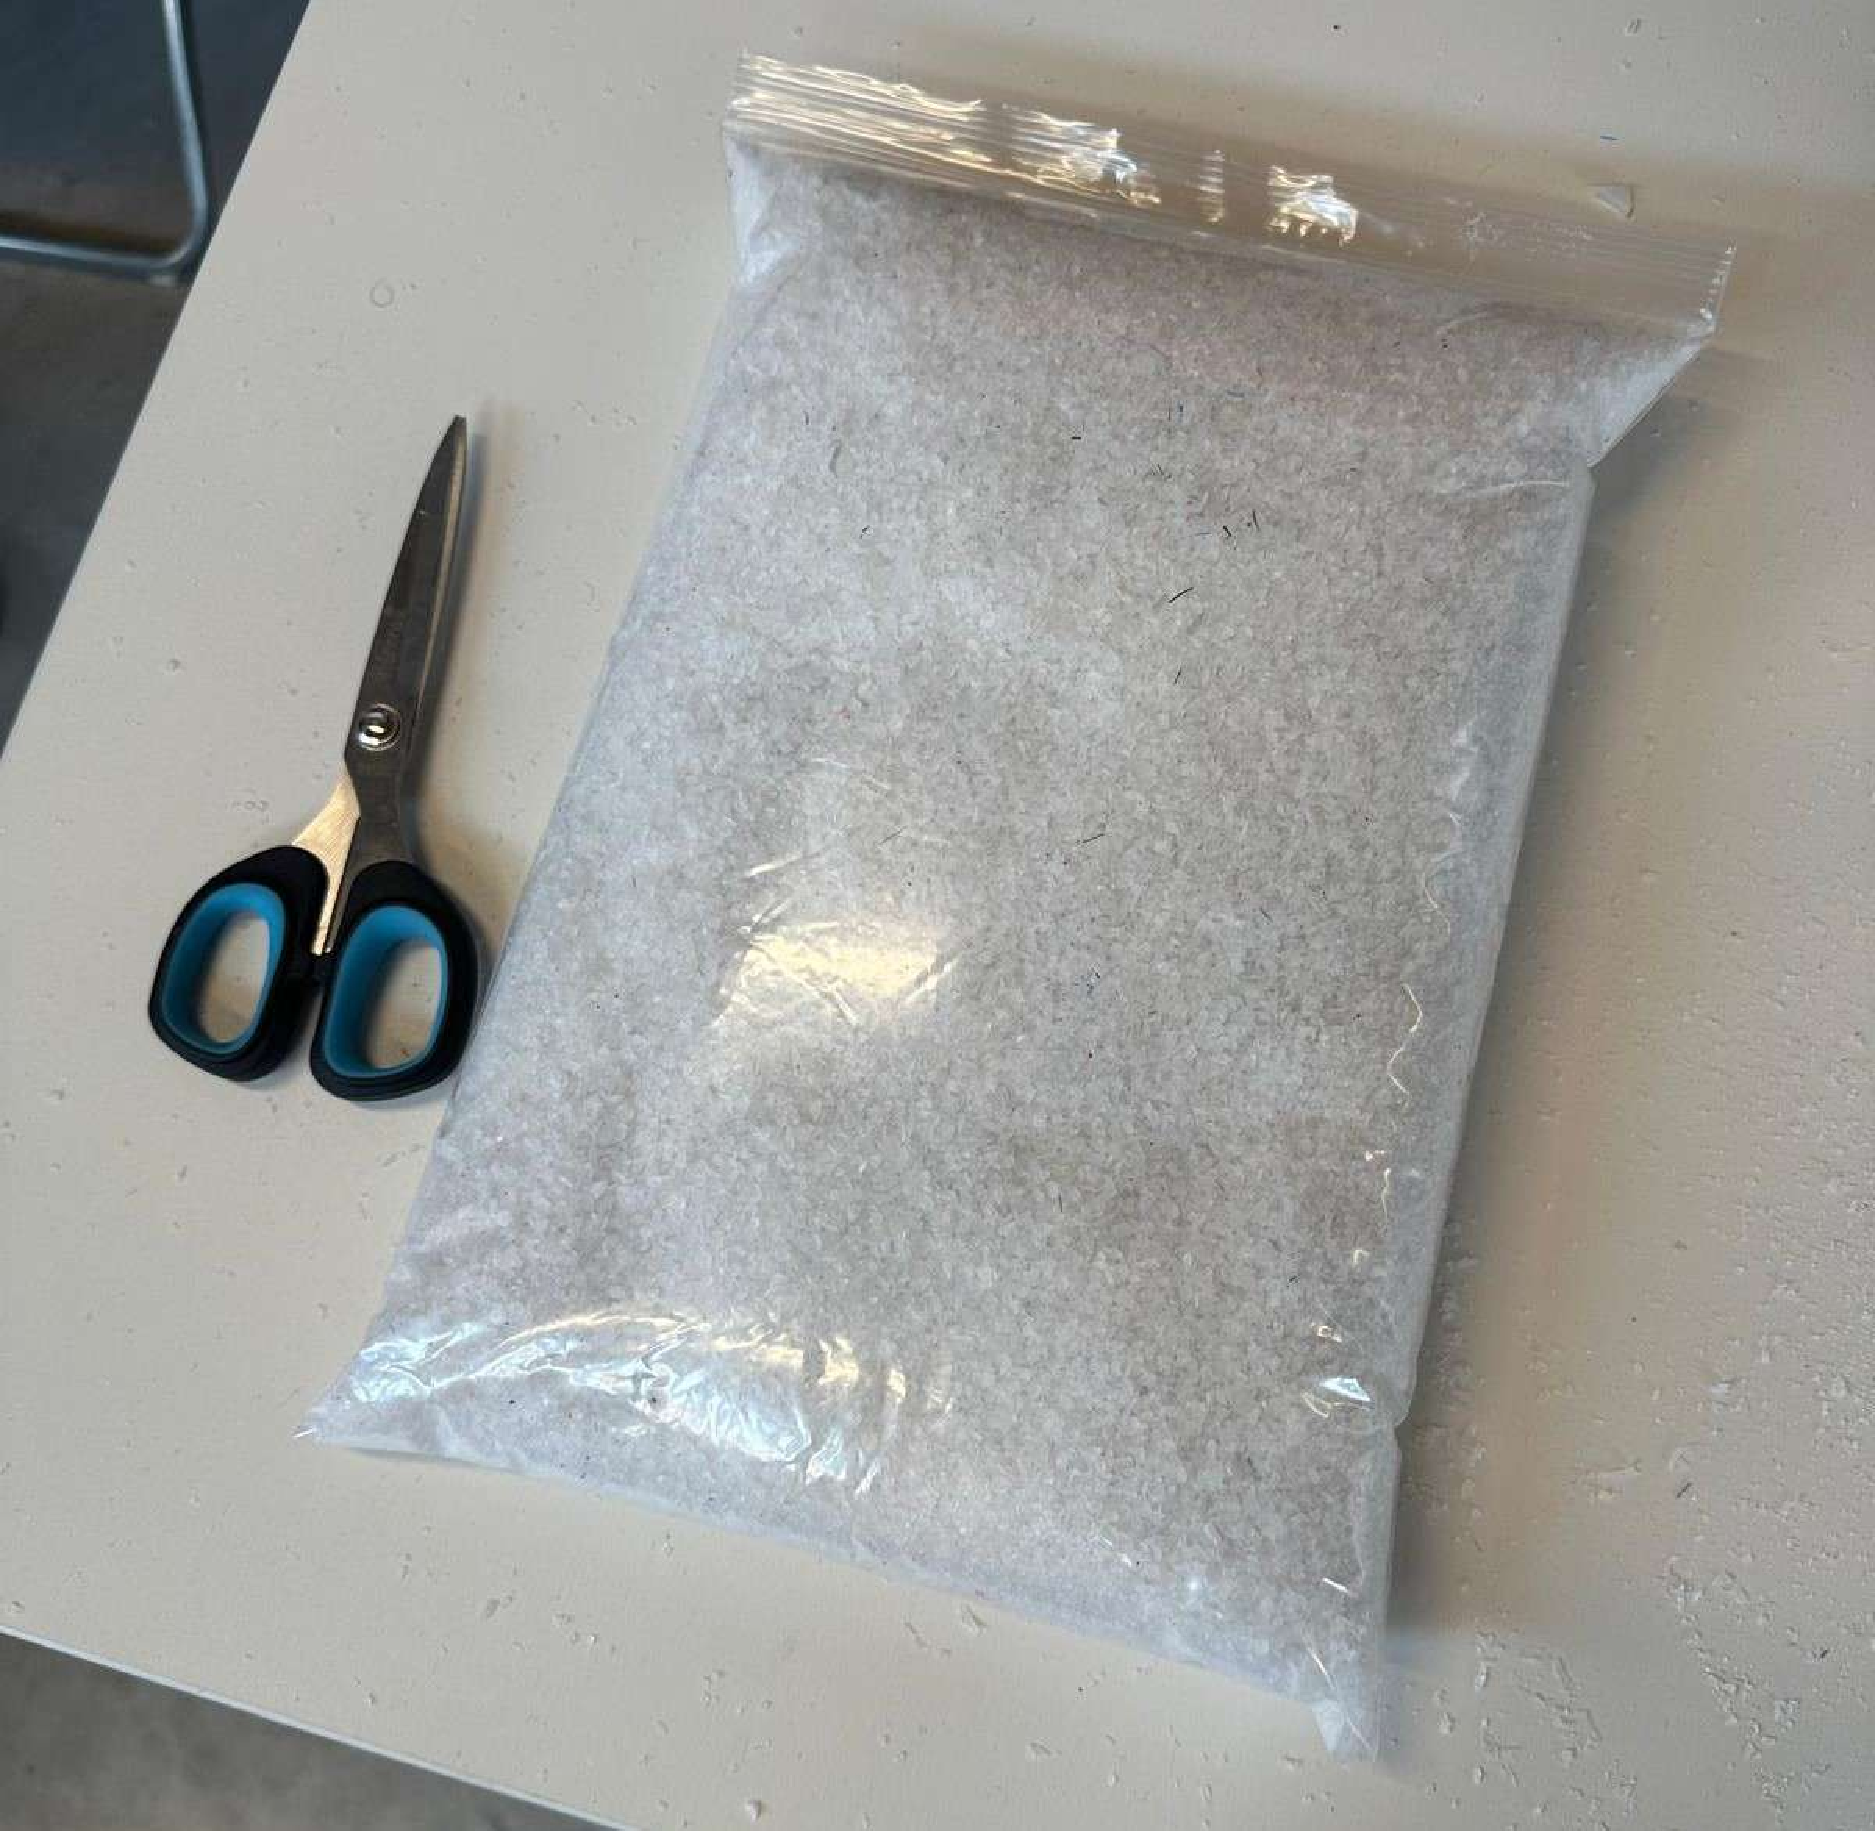
\includegraphics[width = .6\textwidth]{Imagenes/Vectorial/shredded_filament.pdf}
	\caption{Shredded HDPE. Image provided by Gonzalo Alonso García}
	\label{fig:shredded_filament}
\end{figure}

\begin{figure}[h]
	\centering
	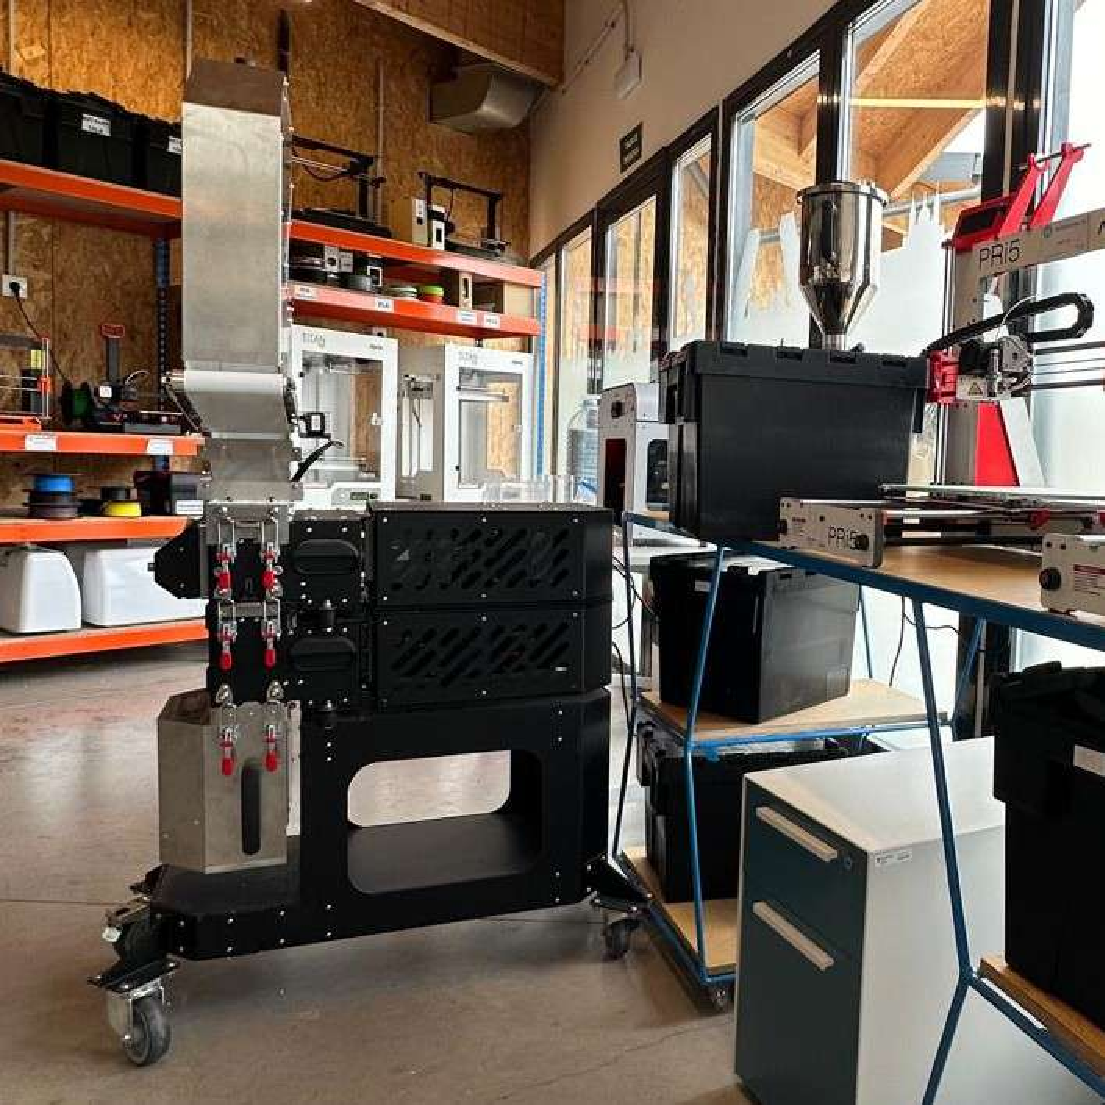
\includegraphics[width = .6\textwidth]{Imagenes/Vectorial/shredder_dryer.pdf}
	\caption{3devo's shredder and dryer. Image provided by Gonzalo Alonso García}
	\label{fig:shredder_dryer}
\end{figure}


\section{Filament Production}
The filament production process was conducted using 3devo's \textit{Filament Maker ONE 
Composer}\footnote{Filament Maker ONE Composer: 
\url{https://www.3devo.com/filament-maker-one-composer-precision}}. This machine is highly 
versatile, allowing fine-tuning through the configuration of numerous parameters. The most 
relevant parameters and their impact on filament quality are detailed below.

\subsubsection*{Extrusion and Filament Diameter}
The filamenting machine is equipped with a sensor that continuously measures the diameter of the 
extruded filament. To maintain a consistent diameter, the machine uses a puller mechanism. This 
puller clamps onto the filament and adjusts its speed: increasing the speed when the filament is 
too thick and decreasing it when the filament is too thin. This adjustment process stretches or 
compresses the filament accordingly to achieve the desired diameter. Additionally, the machine can 
produce a graphical representation of the filament's diameter over time, aiding in the monitoring 
and adjustment process. This graph can be seen in Figure \ref{fig:filament_graph_2}. It can be 
seen that the diamater is fairly unstable, missing by a considerable margin the targets set by the 
two horizontal lines, delimiting the 1.650 and 1.850 millimeters range.

\begin{figure}[h]
	\centering
	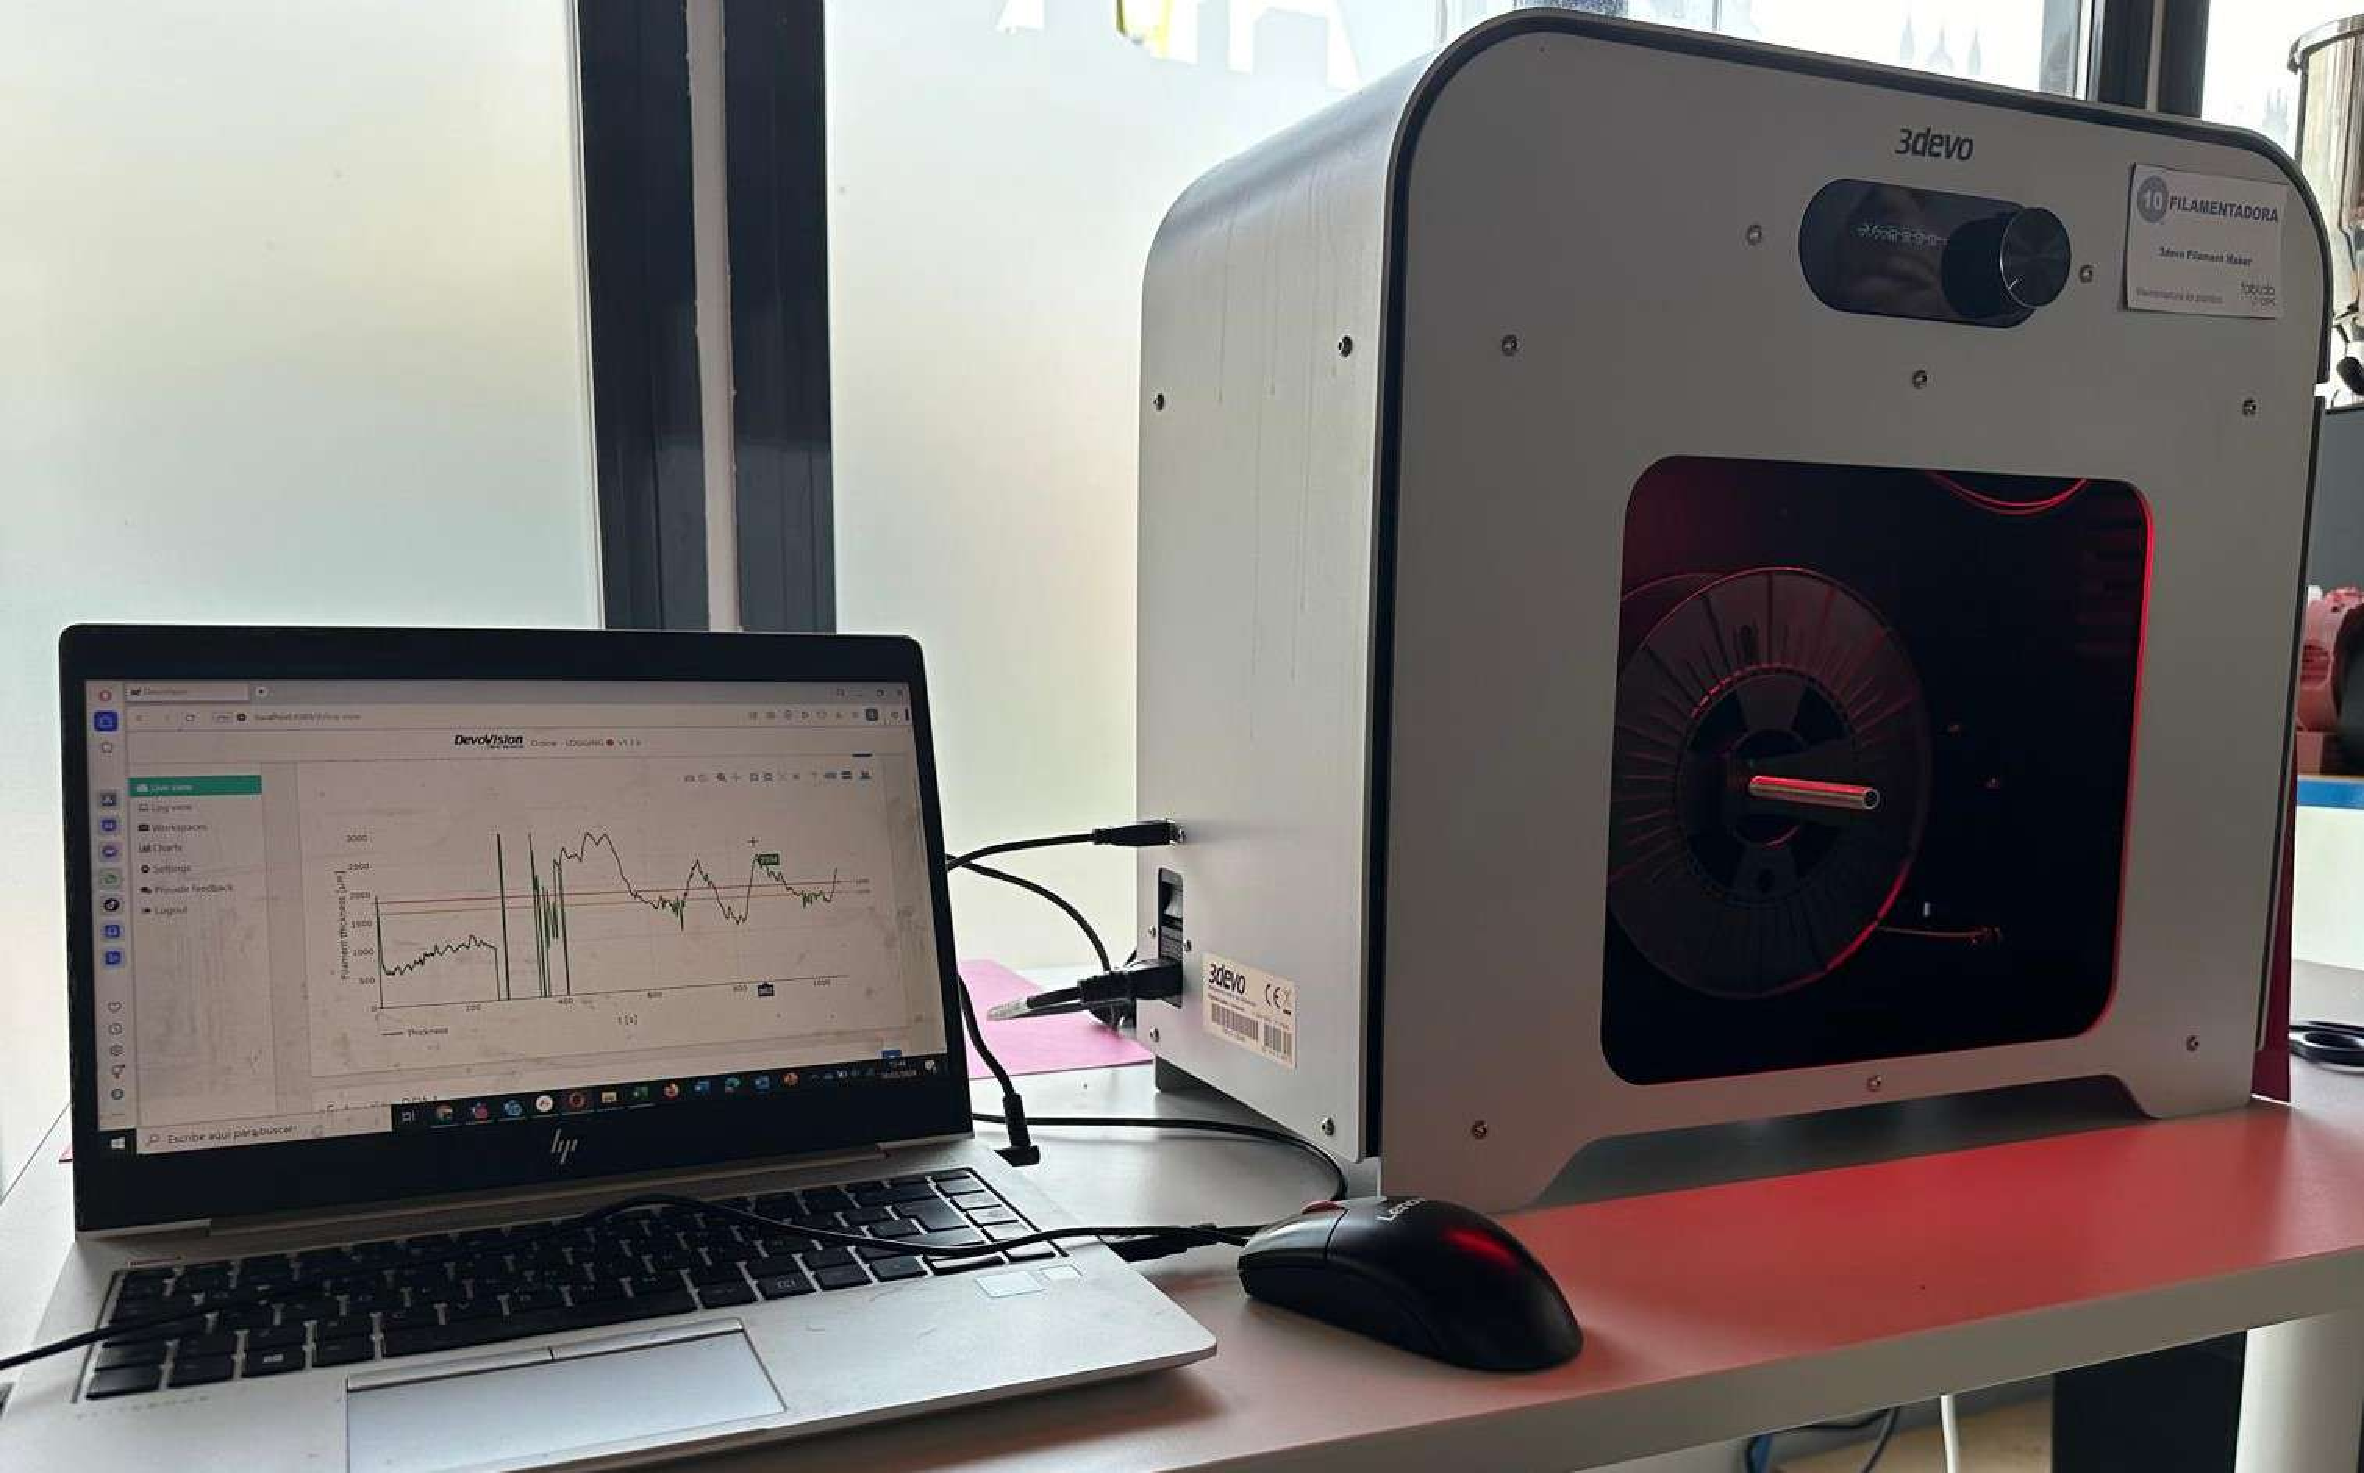
\includegraphics[width = .85\textwidth]{Imagenes/Vectorial/filament_graph_2.pdf}
	\caption{Filament diameter graph with 100\percentsign\ recycled HDPE. Image provided by 
    Gonzalo Alonso García}
	\label{fig:filament_graph_2}
\end{figure}


\subsubsection*{Heaters}
The filamenting machine features four heating zones along an extruder screw that gradually pushes 
the shredded filament through the machine, ultimately extruding it at the end. These heating zones 
are sequentially numbered from 4 to 1, with Zone 4 being the entry point for the shredded plastic 
and Zone 1 being closest to the extruder.

3devo recommends an increasing temperature profile for HDPE, where the temperature is lowest at 
Zone 4 and highest at Zone 1. However, during testing, this setup resulted in an extremely uneven 
filament diameter and a visible texture, indicating incomplete melting and the presence of small 
plastic chunks.

Through extensive experimentation, the team discovered that a decreasing temperature profile 
produced superior results. Starting at approximately 220°C in Zone 4 and reducing the temperature 
to about 170°C in Zone 1 yielded a more consistent and smoother filament. It is speculated that 
this variation in optimal temperature profiles may be due to the recycled nature of the HDPE, 
which alters its melting properties compared to virgin material.

\subsubsection*{Cooling Fans}
Immediately at the extruder's output, two cooling fans are positioned to cool the molten plastic 
as it exits. The speed of these fans needs to be meticulously adjusted to achieve optimal cooling. 
If the plastic is not cooled sufficiently, it remains too soft, causing the puller to crush it. 
Conversely, if the plastic is cooled too much, it becomes too hard, making it difficult for the 
puller to stretch it effectively.

Furthermore, HDPE presents a unique challenge because it consists of two microstructures that 
shrink at different rates when cooled. Rapid cooling can exacerbate this differential shrinkage, 
leading to filament ovalization, a phenomenon where the filament cross-section becomes oval rather 
than circular. This issue is particularly critical because ovalized filament can lead to 
inconsistent extrusion in 3D printers, affecting the quality of the printed parts.

3devo emphasizes the importance of controlled cooling to mitigate these issues\footnote{3devo's 
note on HDPE: \url{https://support.3devo.com/why-is-hdpe-difficult-to-extrude}}. The fans must be 
set to a speed that ensures the plastic is solid enough for handling by the puller but avoids 
rapid cooling that could cause structural inconsistencies. Finding the right balance in fan speed 
is crucial for producing high-quality, round filament that meets the standards required for 
reliable 3D printing. Through careful tuning and testing, the team was able to achieve a cooling 
rate that maintained the filament's integrity and dimensional accuracy.

\section{Challenges and Solutions}

Throughout the filament production process, several challenges emerged. The initial batches of 
extruded filament displayed visible impurities, notably black spots, which resulted in clogging a 
0.4 mm nozzle on the Prusa MK4 3D printer. These impurities are believed to stem from the residual 
dirt on the original plastic containers that were shredded. This underscores the necessity of 
using as-clean-as-possible plastic for shredding to ensure the quality of the final filament.

Another major hurdle was the instability in the filament's diameter. Variations in diameter can 
drastically impact print quality, leading to issues such as under-extrusion when the filament is 
too thin, or even preventing the filament from fitting into the nozzle's 2 mm tube when it is too 
thick. To address this issue, the team experimented with blending virgin HDPE with the shredded 
recycled plastic.

A mixture of 70\percentsign\  recycled HDPE and 30\percentsign\  virgin HDPE yielded significantly 
more stable filament diameter, as illustrated in Figure \ref{fig:filament_graph}. Although a blend 
with 20\percentsign\  virgin HDPE also improved stability, it did not achieve the same level of 
consistency. This blend strategy proved to be a viable solution for mitigating diameter 
instability and improving the overall quality of the filament.

These solutions highlight the importance of both material purity and the strategic use of virgin 
plastic in producing high-quality, reliable 3D printing filament from recycled HDPE. By carefully 
addressing these challenges, the team was able to enhance the performance and usability of the 
recycled filament, paving the way for more sustainable and efficient 3D printing practices.

\begin{figure}[h]
	\centering
	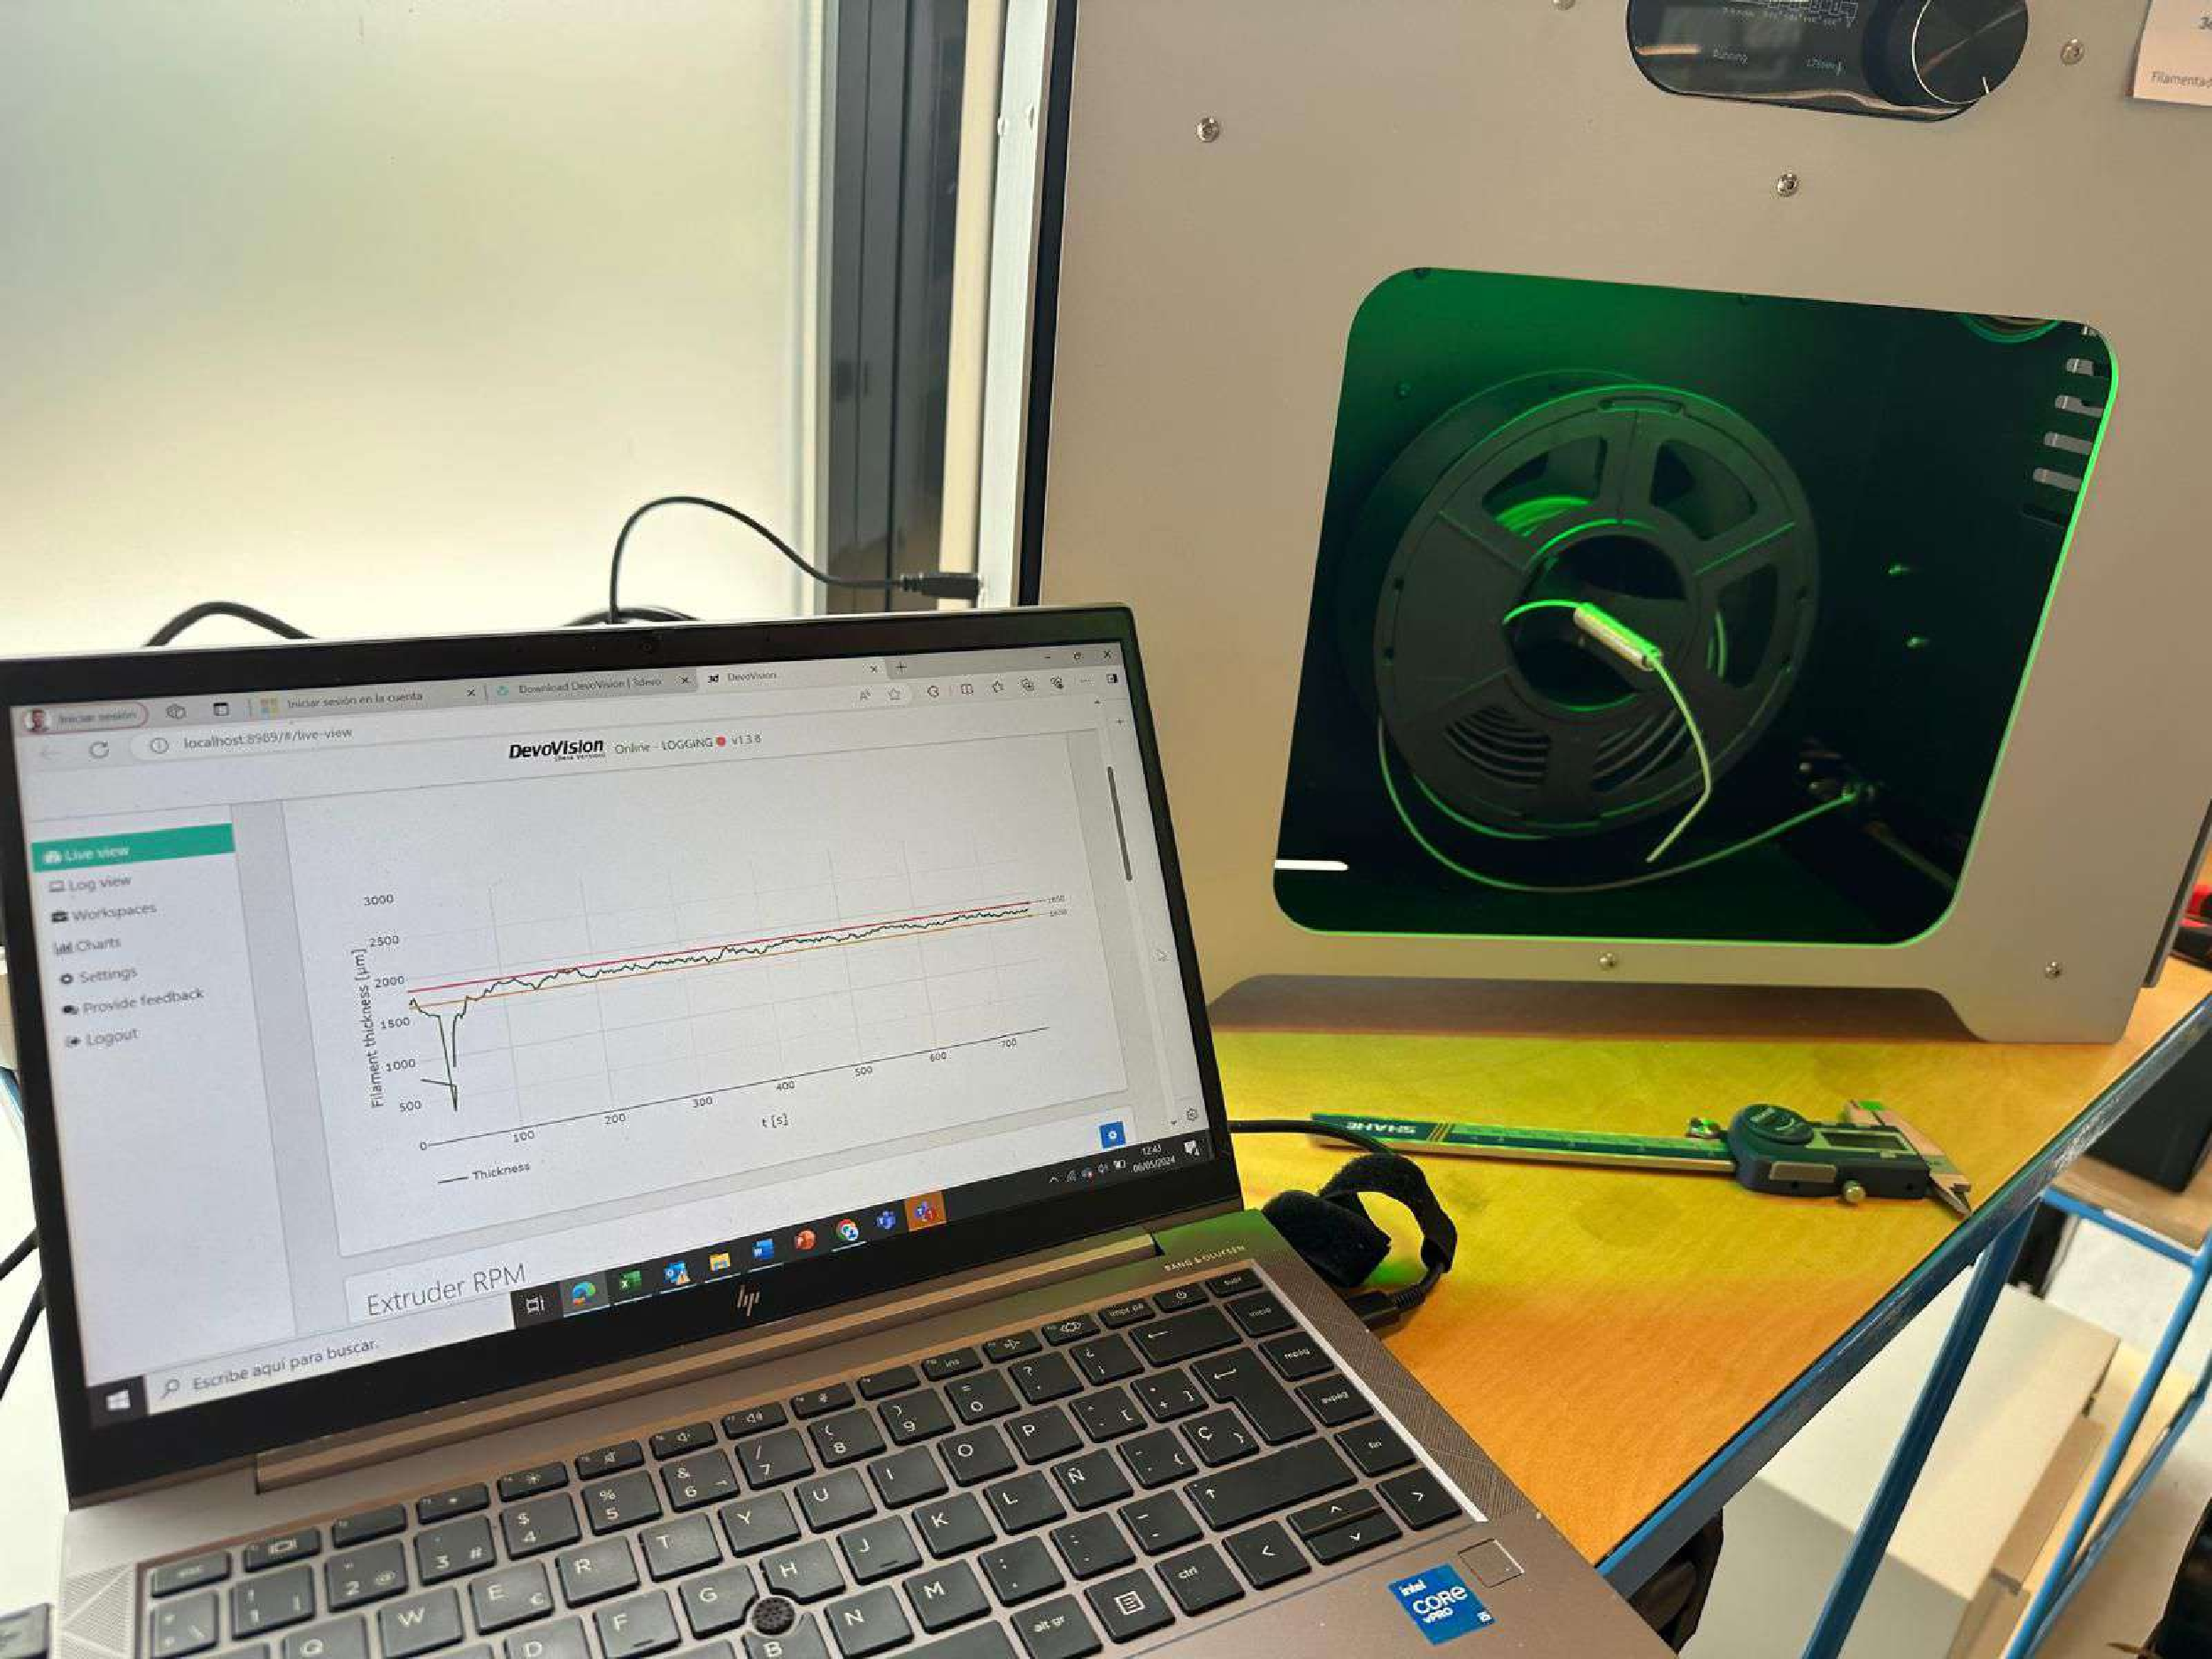
\includegraphics[width = .85\textwidth]{Imagenes/Vectorial/filament_graph.pdf}
	\caption{Filament diameter graph after adding 30\percentsign\ virgin HDPE. Image provided by 
    Gonzalo Alonso García}
	\label{fig:filament_graph}
\end{figure}

\section{Conclusions}
In conclusion, the exploration of recycling HDPE for 3D printing filament has been both 
challenging and enlightening. The initial stages of filament production highlighted critical 
issues such as impurities and diameter instability, both of which were addressed through 
meticulous preparation and the addition of virgin HDPE. These steps ensured a cleaner, more 
consistent filament suitable for 3D printing.

Despite the early setback of a clogged nozzle, the groundwork has been laid for further 
experimentation with 3D printing using this recycled filament. The next phase involves testing the 
printability of HDPE, addressing potential challenges such as warping and adhesion problems that 
are commonly associated with this material. With the setup now optimized, future trials will focus 
on overcoming these obstacles to fully realize the potential of recycled HDPE in 3D printing 
applications.

The collaboration with the Sustainability team and the support from the ``Centro de Innovación en 
Economía Circular'' have been invaluable, demonstrating the feasibility and benefits of 
integrating circular economy principles into technological projects.
